\title{Umělá inteligence}

\section{Umělá inteligence(UI) - Definice, úzká UI obecná UI, superinteligence, strojové učení}
Umělá intelgince je výpočetní systém vykonávající činnost, kterou si spojujeme s lidskou inteligencí\\
Další definice: 
\begin{itemize}
    \item počítačové systémy, které jsou schopné plnit úkoly, které obvykle vyžadují lidskou inteligenci, jako je rozhodování, detekce objektů, řešení složitých problémů
    \item vědní disciplína, zabývající se teoríí systémů zpracovávajících data a schopných se víceméně samostatně rozhodovat
    \item schopnosti počítače/algoritmu napodobovat/realizovat některé funkce lidského mozku
\end{itemize}
\subsection*{Úzká umělá inteligence}
stupeň UI zahrnující stroje, které mohou provádět pouze úzce definovaou sadu konkrétních úkolů\\
jediná forma, které lidstvo doposud dosáhlo\\
aplikace na rutinních pracích - rozpoznávání řeči, obrazu, počítačové vidění, inteligentní budovy, hra šachů, návrh nákupu, počasí\\
UI je vznešený název pro sofistikované SW řešení, vkládáme důvěru do autora, že nic neopomenul\\
\begin{figure}[H]
    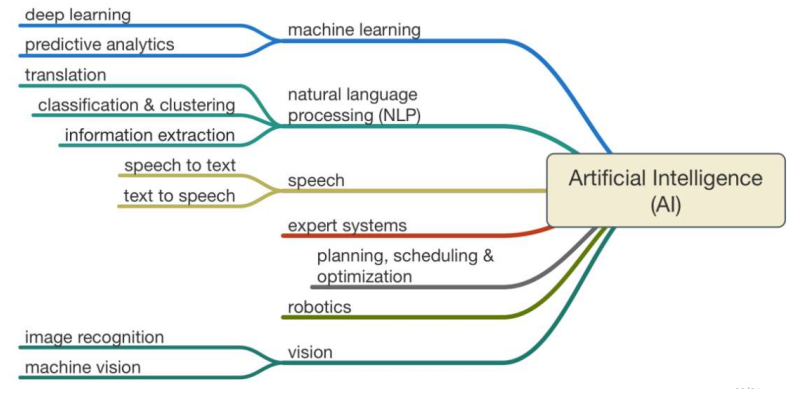
\includegraphics[scale = 1]{images/uzkeAI.png}
\end{figure}
\subsection*{Obecná UI}
Umělá inteligence na úrovni člověka\\
umí se rozhodovat, komunikovat, samostatně se učit\\
zatím není vyvinuta\\
Tuninguv test - nemožnost rozeznat člověka od stroje\\

\subsection*{Superinteligence}
má vyšší inteligenci než člověk\\
uvědomuje si, že ji ovládají a omezují intelektuálně podřadní lidé\\



\subsection*{Strojové učení(machine learning)}
\begin{itemize}
    \item zaměření na to, aby se stroje rozohodovaly na základě dat
    \item techniky strojového učení:
    \item \begin{itemize}
        \item učení s učitelem
        \item učení bez učitele
        \item zpětnovazební učení, posílené učení
    \end{itemize}
\end{itemize}
Učení s učitelem:
\label{typ_uceni}
\begin{figure}[H]
    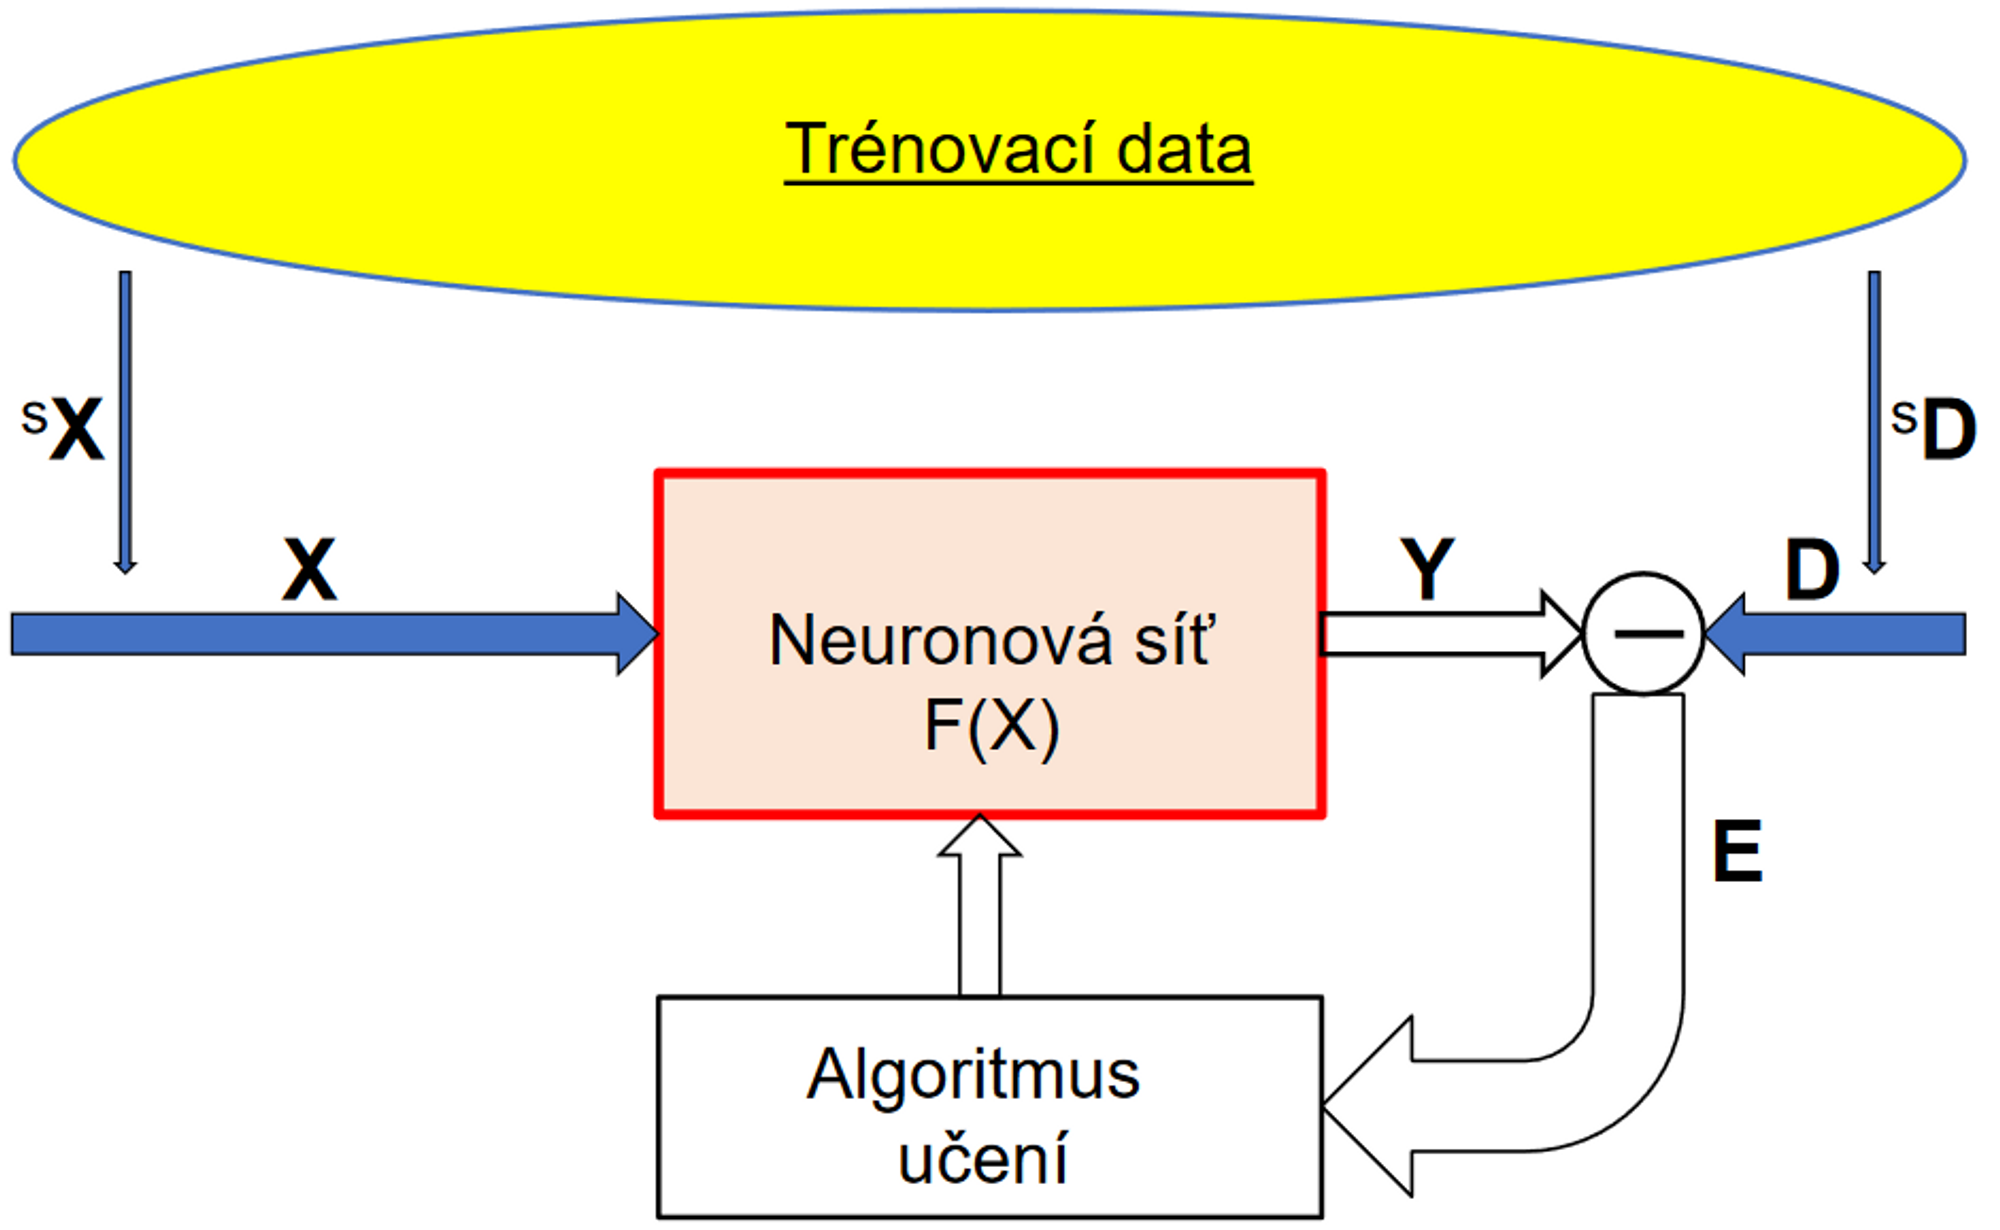
\includegraphics[scale = 0.3]{images/sUcitelem.png}
\end{figure}
Data jsou rozdělena na trénovací, validační a testovací\\
Učení probíhá tak, že systému předkládáme trénovací vzory a zároveň požadované výstupy, na základě kterých se mění váhy.\\
\newpage
Učení bez učitele:
\begin{figure}[H]
    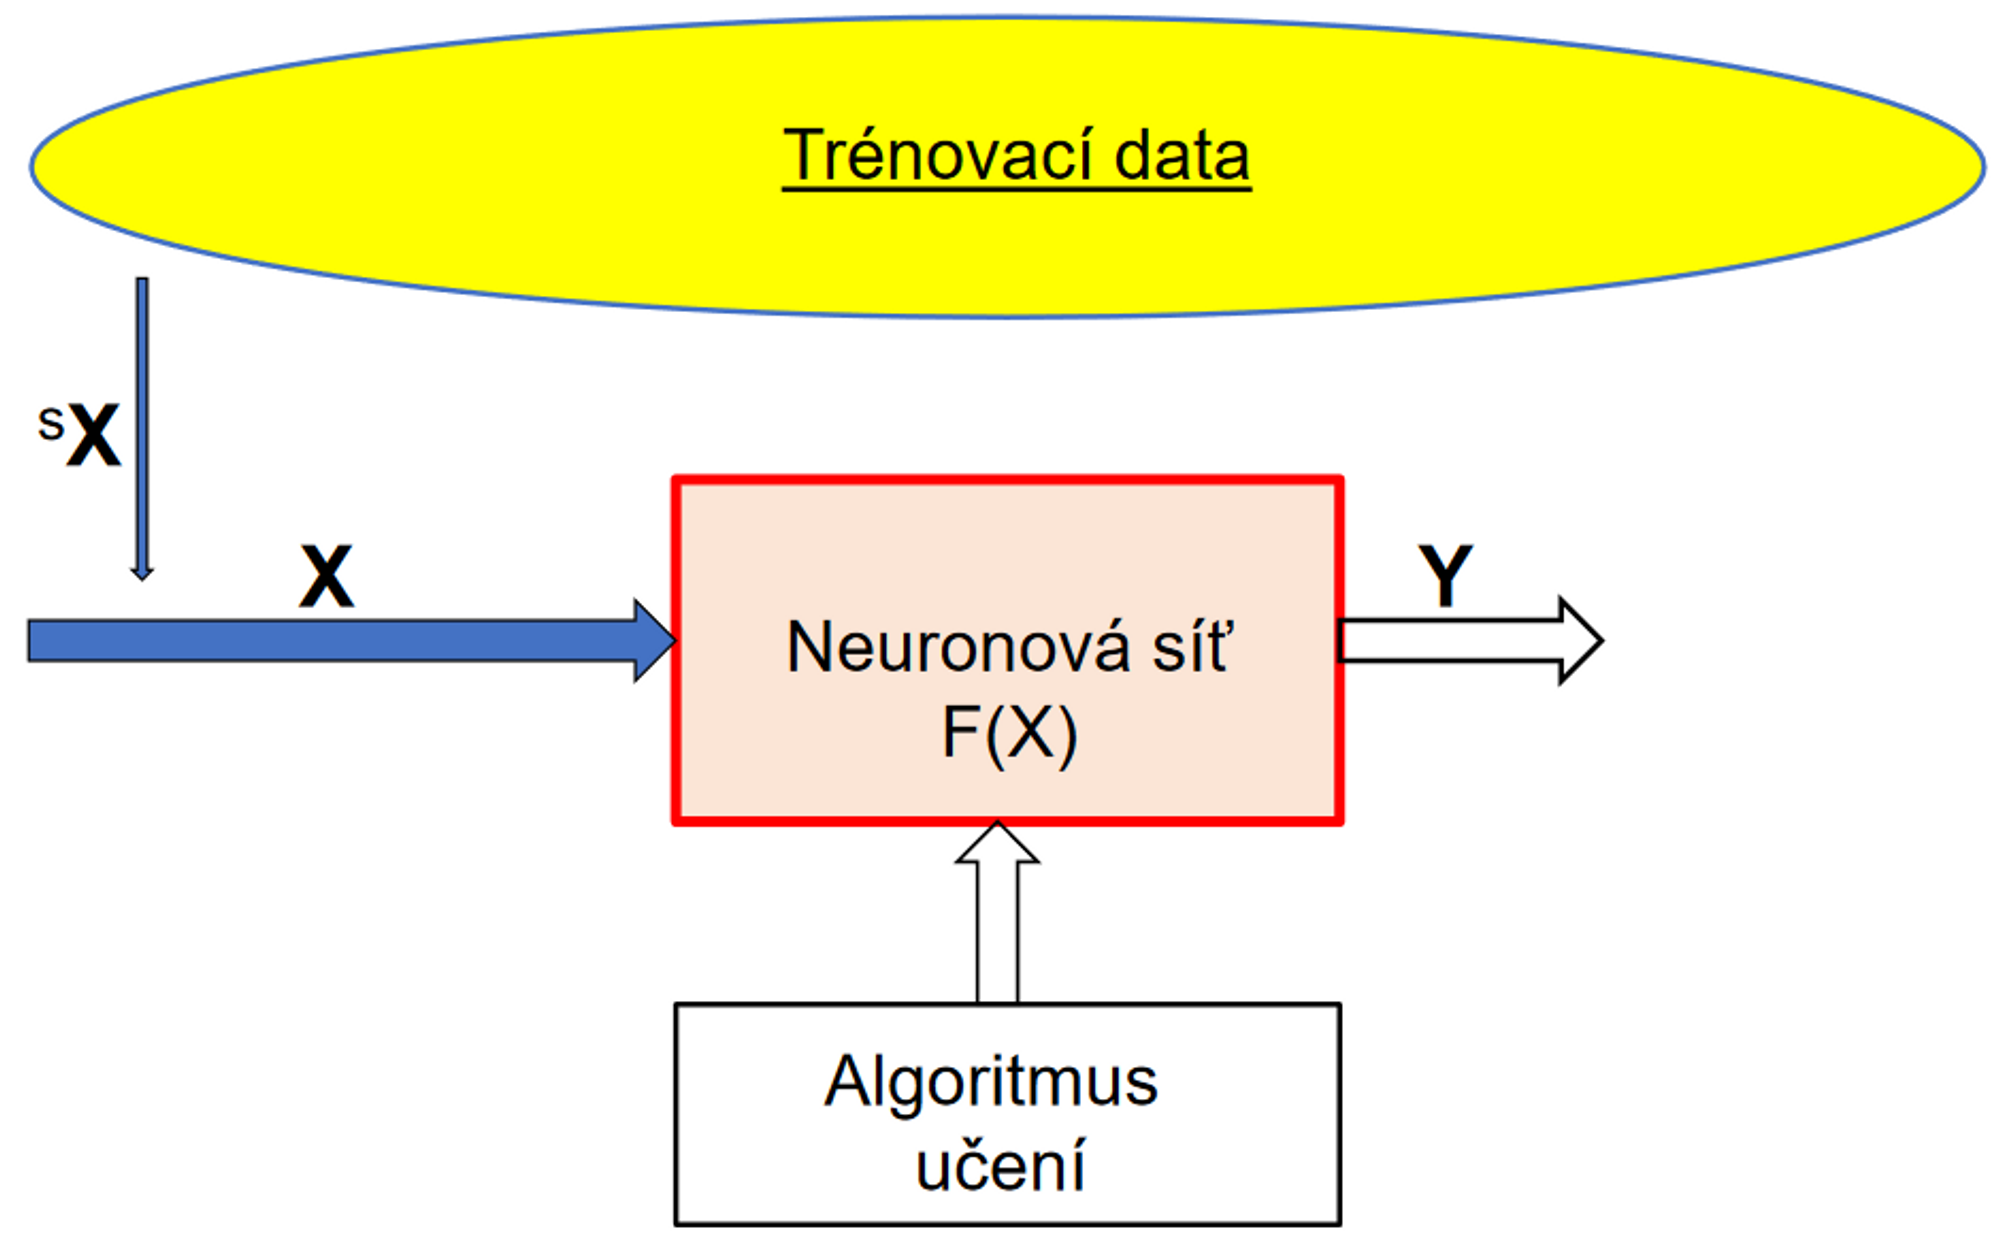
\includegraphics[scale = 0.4]{images/bezUcitele.png}
\end{figure}
Data jsou pouze jednoho typu a to trénovací\\
Učení probíhá tak, že jsou systému předloženy sady vstupů(bez správných výsledků, protože je neznáme) a na základě vstupů se mění váhy.\\

Existuje i kombinace obou přístupů, nazývá se expectation maximization algoritmus.

\subsection*{Základní druhy úloh}
\begin{itemize}
    \item Klasifikace vstupních dat do tříd
    \item Odhadování výstupní hodnoty podle vstupu
    \item Zařazování objektů do skupin podle podobných vlastností - učení bez učitele
\end{itemize}

\section{Umělé neuronové sítě - paradigmata, perceptron, algoritmus Backpropagation, Kohonenova samoorganizační mapa, konvoluční neuronová síť}
\subsection*{Paradigmata}
použité modely neuronů\\
topologie\\
způsob učení\\
způsob vybavování\\

\subsubsection*{Neuron}
\begin{figure}[H]
    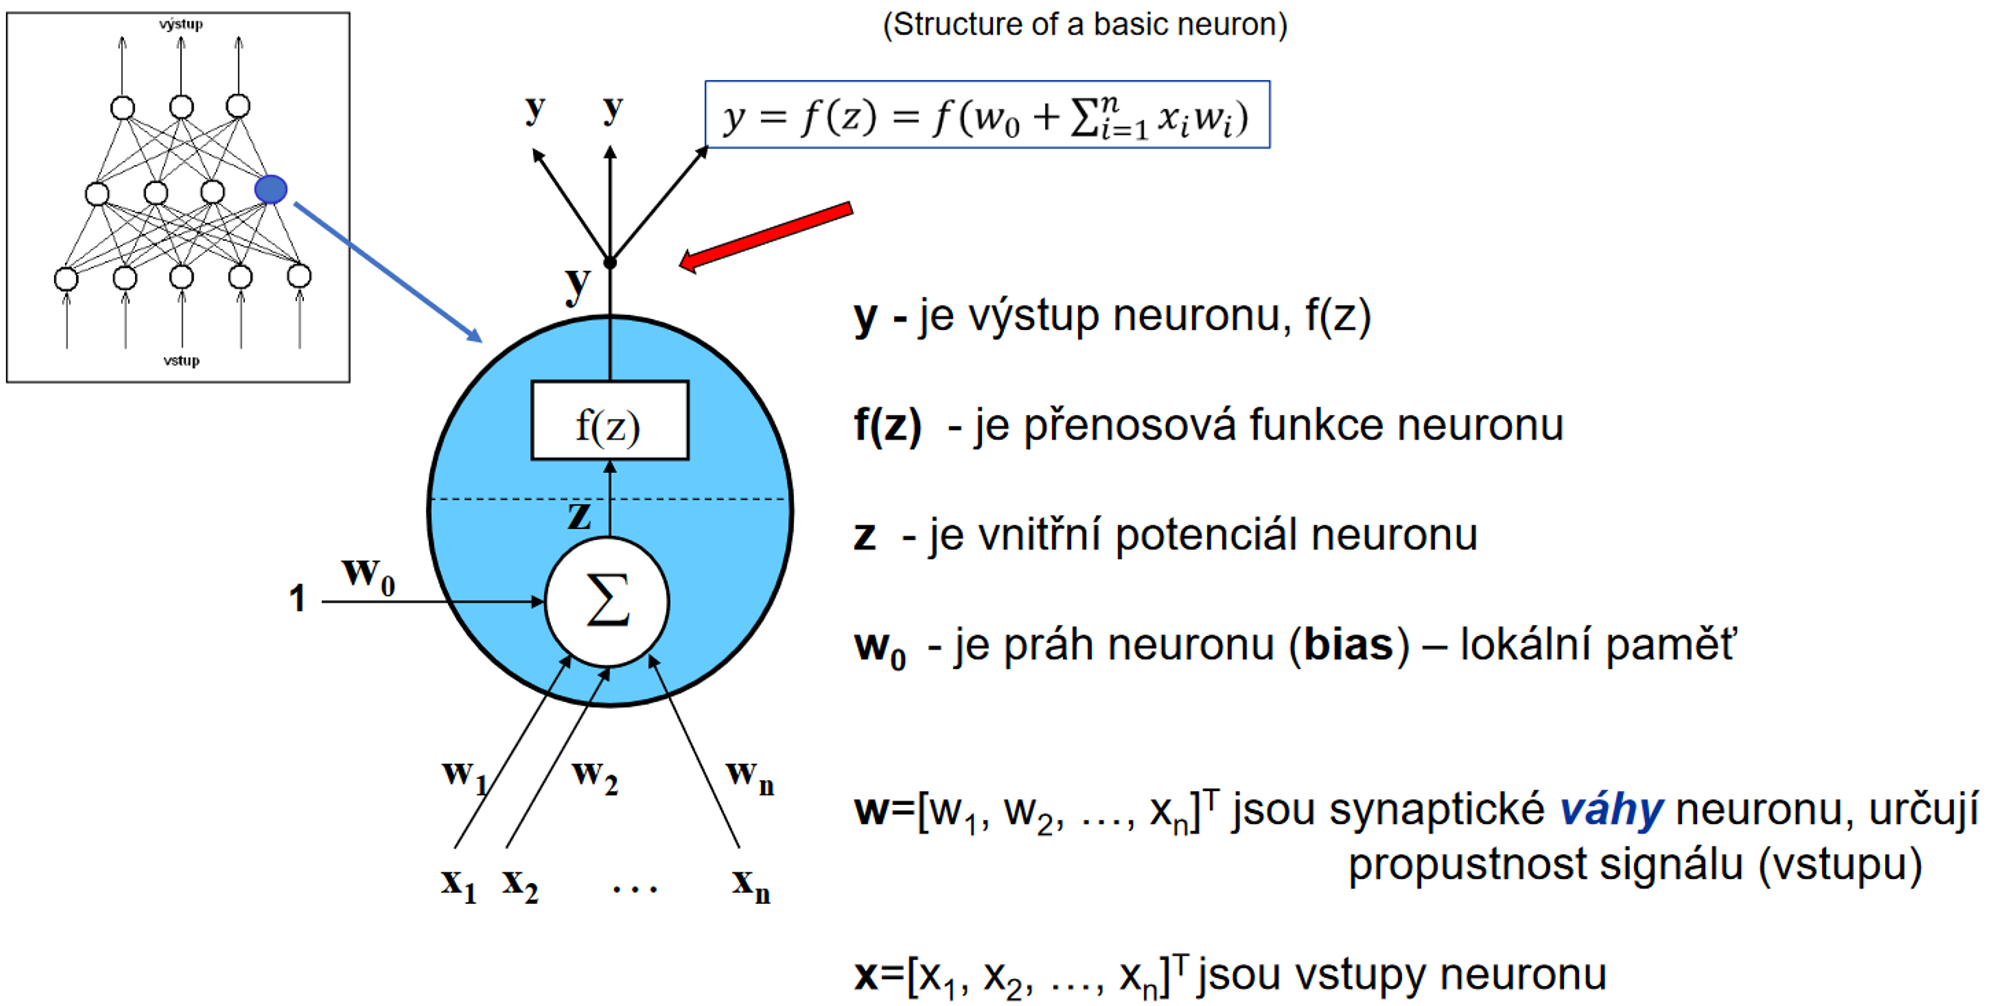
\includegraphics[scale = 0.5]{images/neuron.png}
\end{figure}
vnitřní potenciál neuronu je lineární, nebo radiální
\begin{itemize}
    \item lineární: $z = w_0 + \sum^n_{i=1}x_iw_i$
    \item radiální: $z = w_0 + \sqrt{\sum^n_{i=1}(x_i-w_i)^2}$
\end{itemize}

\subsubsection*{Topologie}
Orientovaný graf
\begin{itemize}
    \item neurony tvoří uzly grafu
    \item hrany grafu se nazývají spoje 
    \item každý spoj má váhu
    \item každý neuron má libovolný počet vstupů a výstupů(stejných)
    \item každý neuron má bias, vnitřní potencíál a přenosovou funkci
\end{itemize}
struktura je Přímovazební nebo zpětnovazební:
\begin{figure}[H]
    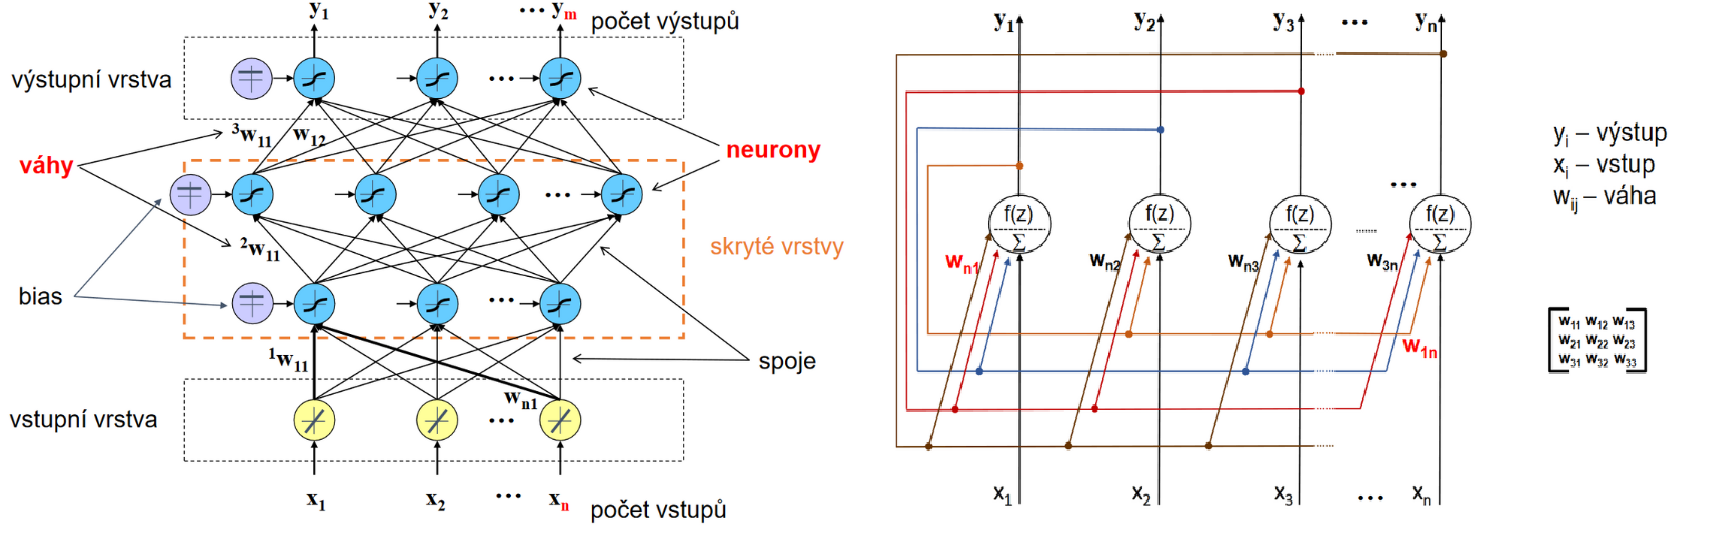
\includegraphics[scale = 0.5]{images/struktury.png}
\end{figure}

\subsubsection*{Učení popsáno v předchozí otázce viz \ref{typ_uceni}}

\subsubsection*{Vybavování}
aktivní režim\\
vlastní výpočet funkce naučené neuronové sítě na daný vstup\\
jsou dva typy:
\begin{itemize}
    \item jednorázový - přímovazební, odezva probíhá v jedné iteraci
    \item iterační proces - zpětnovazební, odezva probíhá iterativně
\end{itemize}

\subsubsection*{Aplikace}
regrese - predikce spojité proměnné na základě vstupu\\
klasifikace - zařazení do tříd(detekce spamu, jestli poslat pacienta na dané vyšetření)\\
časové řady - jak regrese tak klasifikace\\
shluková analýza - učení 

\subsection*{Perceptron}
Charakteristika:
\begin{itemize}
    \item neuron - nespojitá přenosová funkce
    \item topologie - jednovrstvá přímovazební
    \item učení - iterativní, s učitelem
    \item tréninková množina - \textbf{lineárně separabilní}
    \item vybavování - jednorázový proces
    \item aplikace - lineárně separabilní klasifikátor
\end{itemize}
\subsubsection*{Neuron}
\begin{figure}[H]
    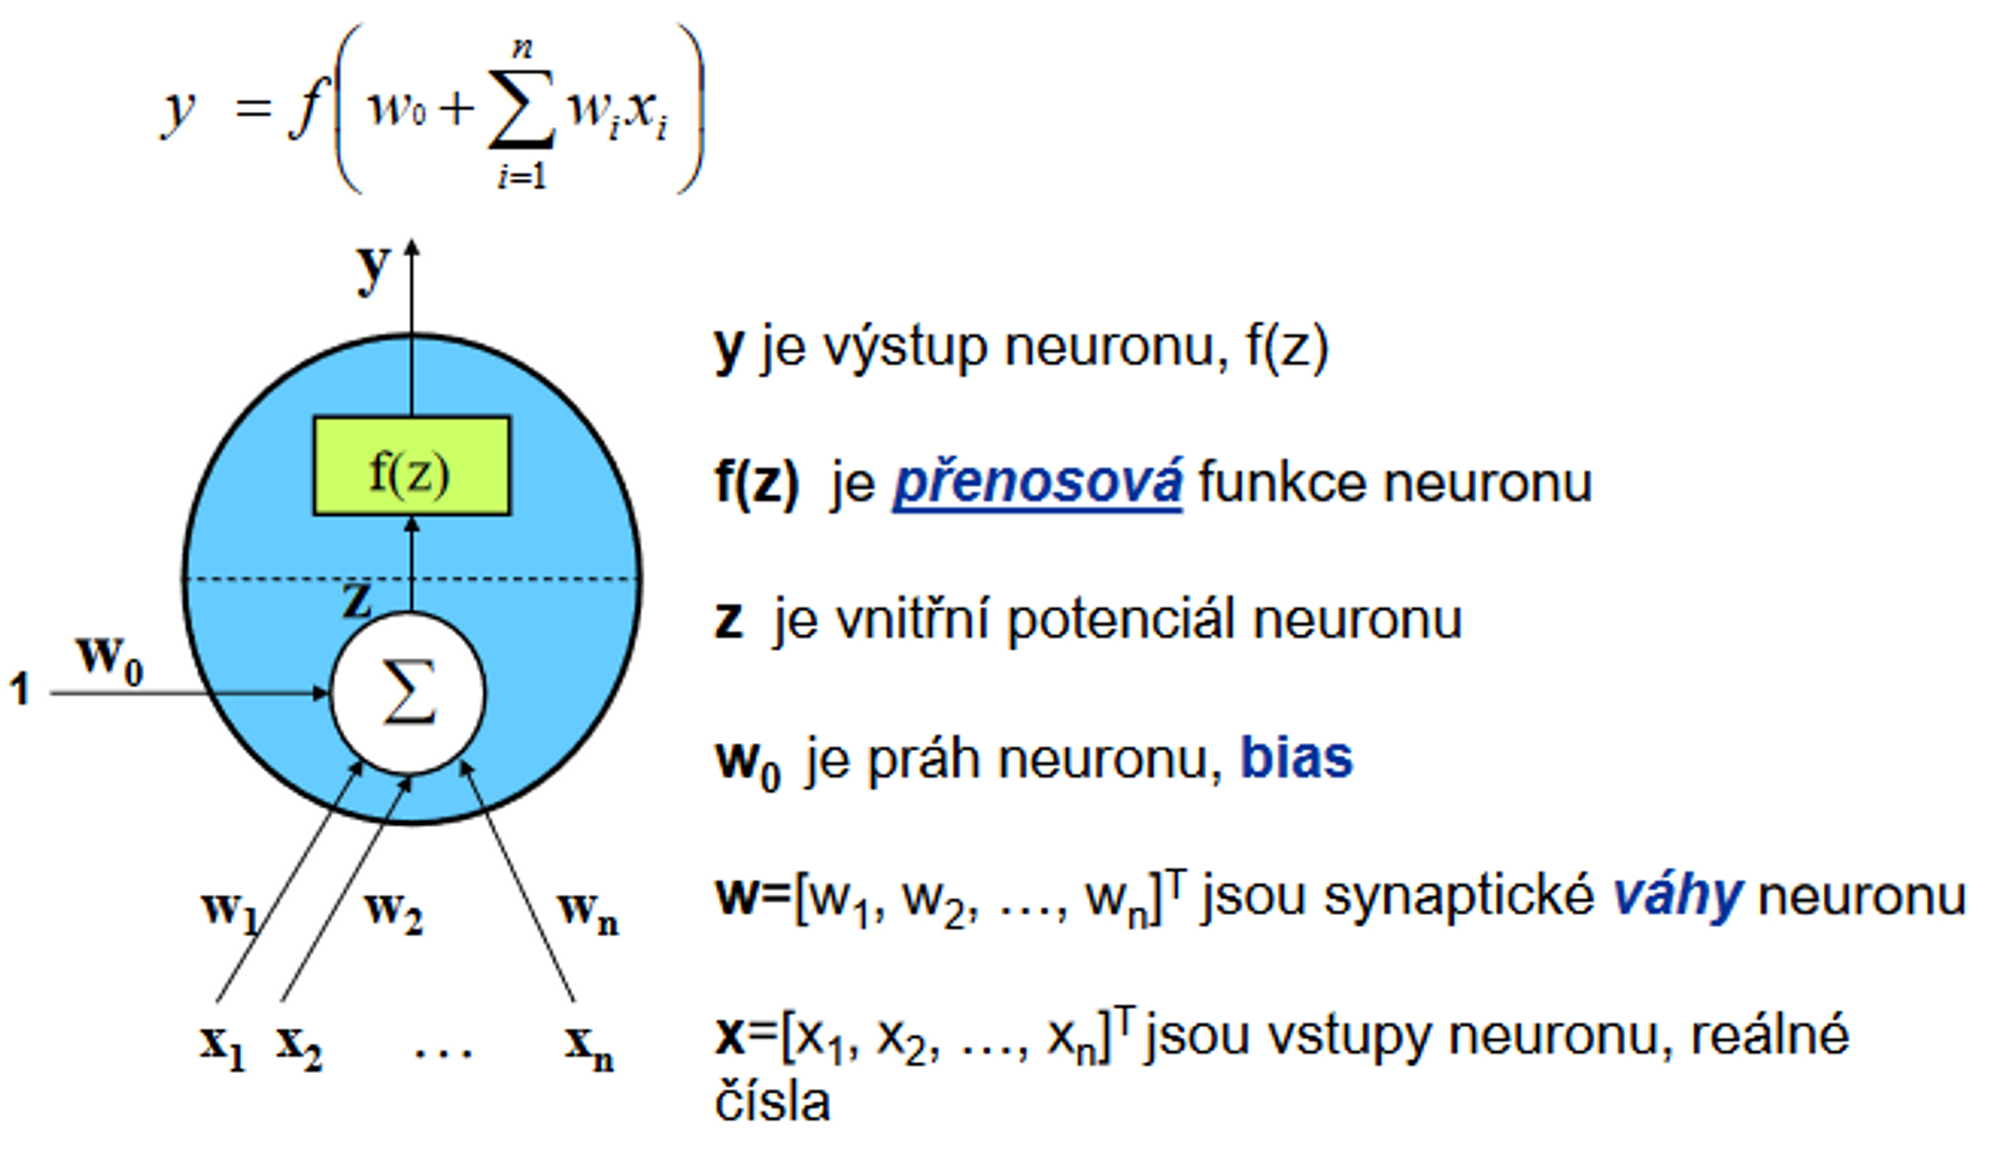
\includegraphics[scale = 0.3]{images/perceptron_neuron.png}
\end{figure}
\newpage
Přenosová funkce bez prahu:
\begin{figure}[H]
    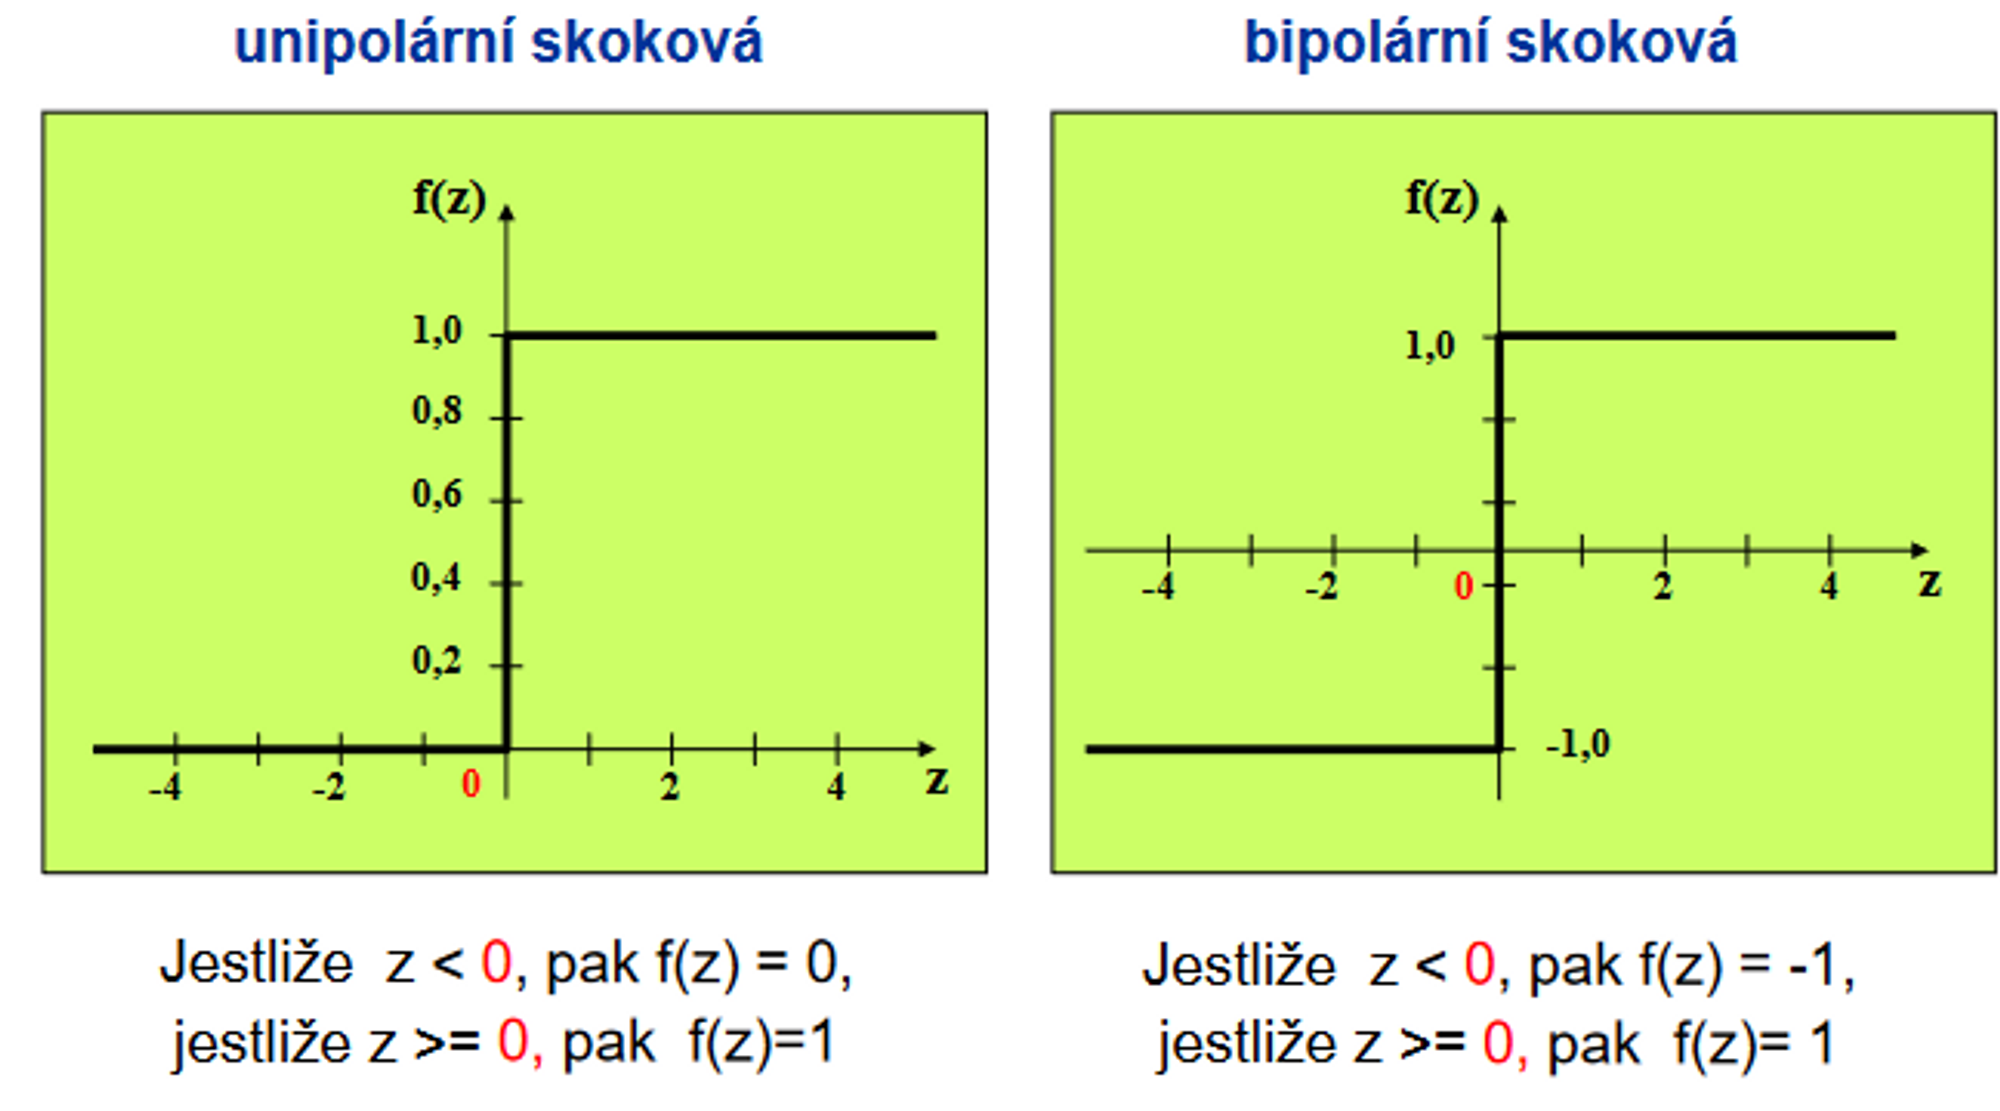
\includegraphics[scale = 0.3]{images/perceptron_prenos.png}
\end{figure}
Přenosová funkce s prahem
\begin{figure}[H]
    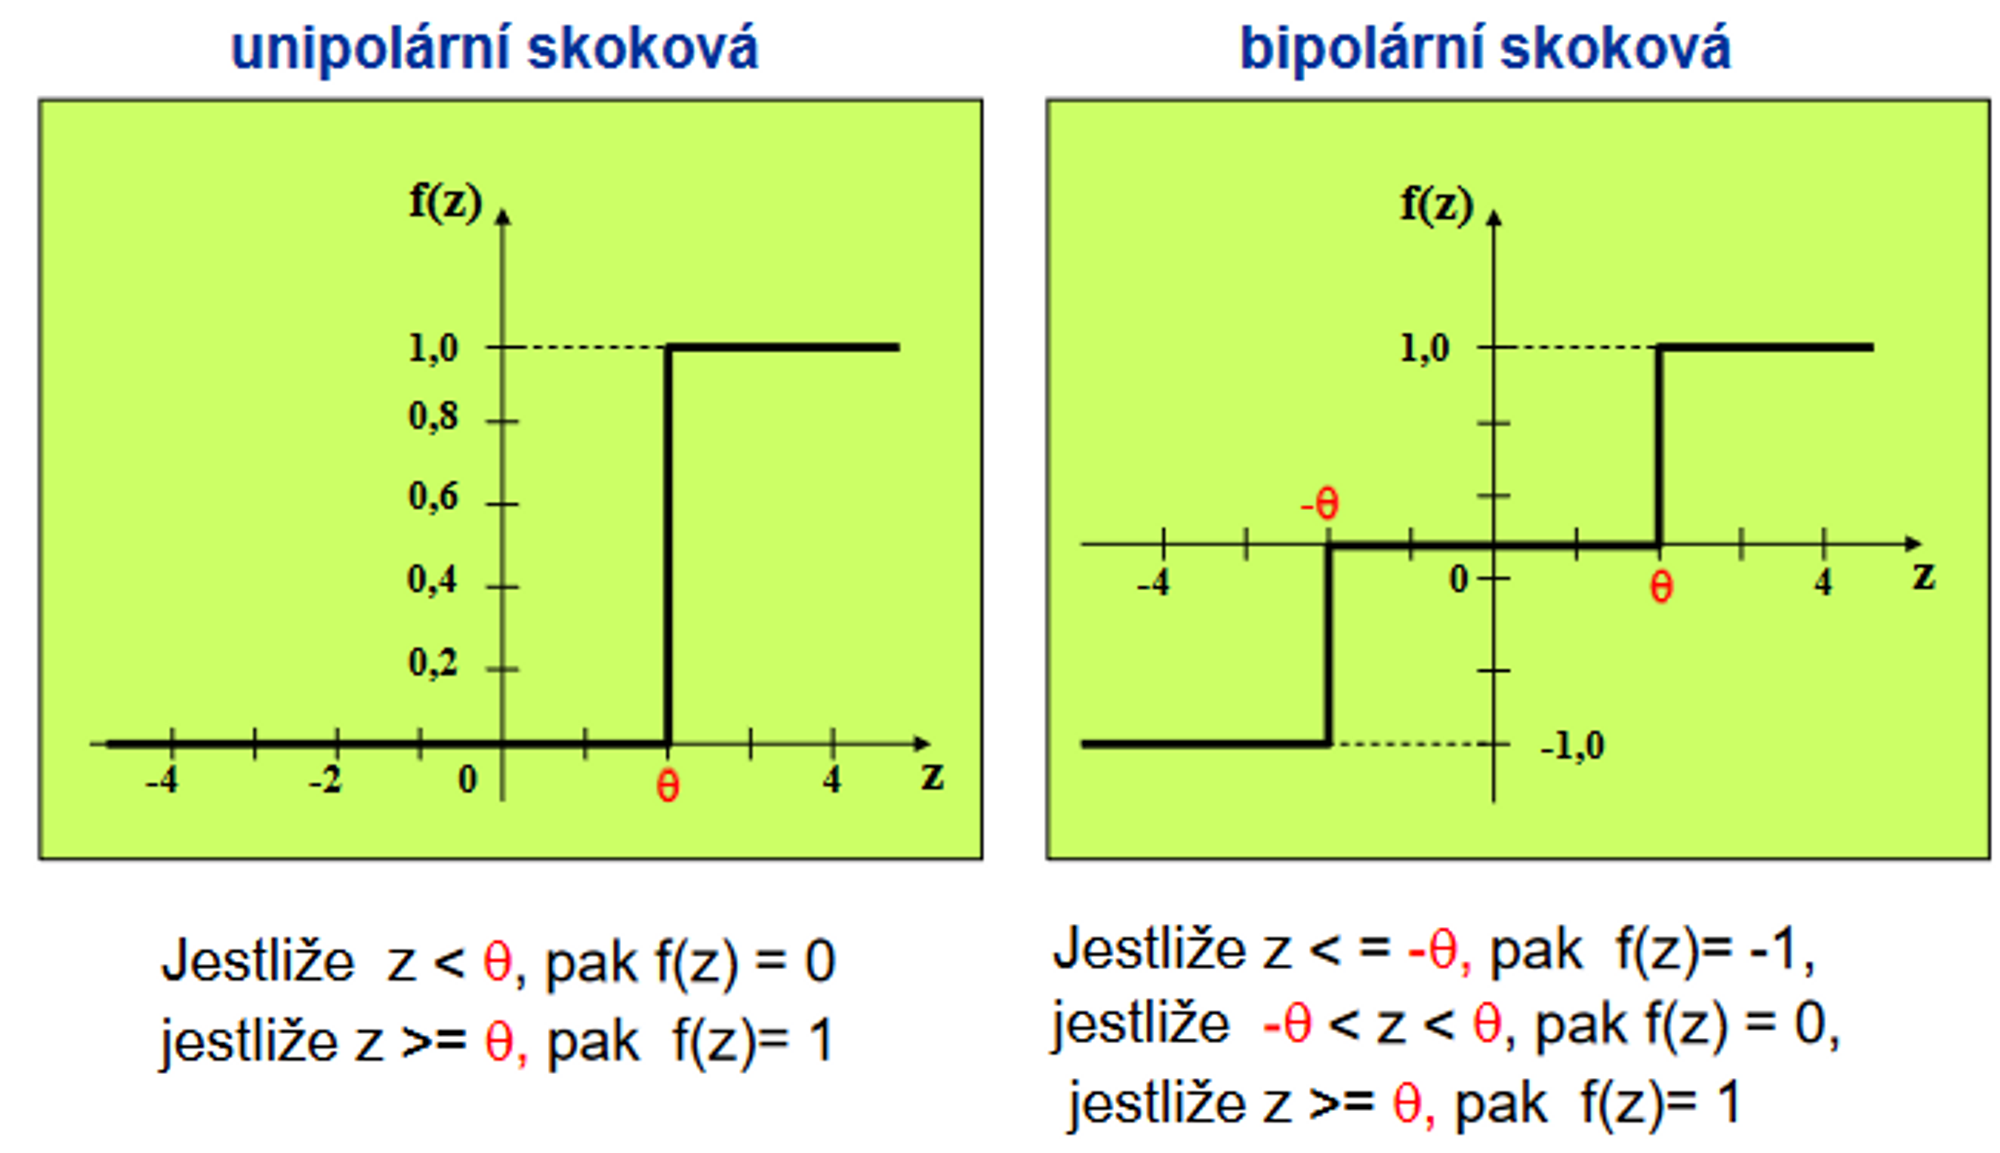
\includegraphics[scale = 0.3]{images/perceptron_prenos_s_prahem.png}
\end{figure}

\subsubsection*{Topologie}
jeden nebo více perceptronů
\newpage
\subsubsection*{Učení}
když je v n-rozměrném rostoru lineárně separabilní třída objektů, v konečném počtu kroků učení lze najít vektor vah perceptronu, který je oddělí\\
Kroky učení:
\begin{enumerate}
    \item Start, inicializace(nastavení vah a určení přenosové funkce)
    \item předložení tréninkového vzoru
    \item výpočet výstupu sítě
    \item učení - adaptace vah
    \item test na shodu
    \item test na ukončení - jestli jsou všechny klasifikace správně
\end{enumerate}
Nastavení vah je na malá náhodná čísla\\
Adaptace vah probíhá třemi různými způsoby:\\
A):
\begin{figure}[H]
    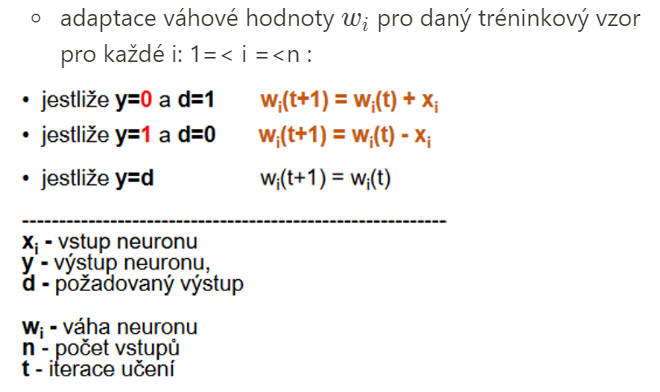
\includegraphics[scale = 1]{images/perceptron_vahy1.png}
\end{figure}
\newpage
B):
\begin{figure}[H]
    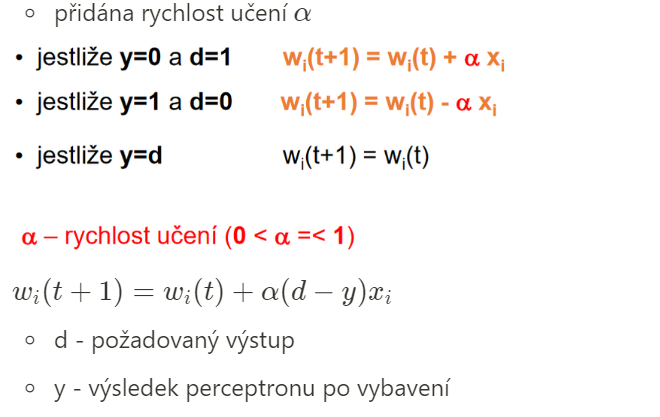
\includegraphics[scale = 1]{images/perceptron_vahy2.png}
\end{figure}
C):
\begin{figure}[H]
    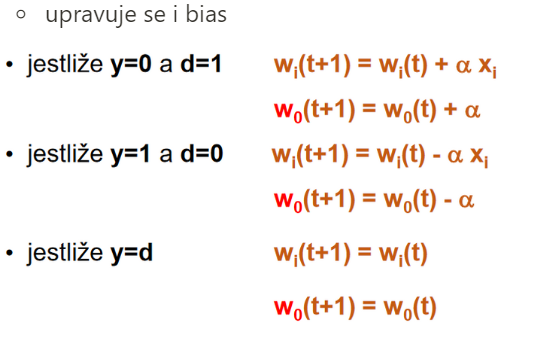
\includegraphics[scale = 1]{images/perceptron_vahy3.png}
\end{figure}

\subsubsection*{vybavování}
Výstup:
\begin{itemize}
    \item 0/1
    \item -1/1
    \item -1/0/1
\end{itemize}
\subsubsection*{Kritika perceptronu}
schopný řešit jen problémy, které jsou linárně separabilní\\
nelze realizovatfunkci XOR

\subsection*{Algoritmus Backpropagation}
Charakteristika
\begin{itemize}
    \item neuron - spojitá přenosová funkce
    \item topologie - vícevrstvá, přímovazební
    \item učení - s učitelem, iterační gradientní proces nastavení vah, algoritmus se zpětným šířením chyby
    \item vybavování - jednorázový proces
    \item aplikace - modelování nelineárních funkcí, klasifikace
\end{itemize}

\subsubsection*{Neuron}
ve vstupní vrstvě distribuce signálu, přenosová funkce lineární(nemusí mět strmost 1)\\
ostatní vrstvy přenosová funkce sigmoida(výstup 0/1), tangenta hyperbolická(-1/1)

\subsubsection*{Topologie}
minimálně 3 vrsty neuronů\\
vstupní vrstva - distrubuce signálu\\
prostřední vrstvy(skryté) - úplné propojení neuronů\\
\begin{figure}[H]
    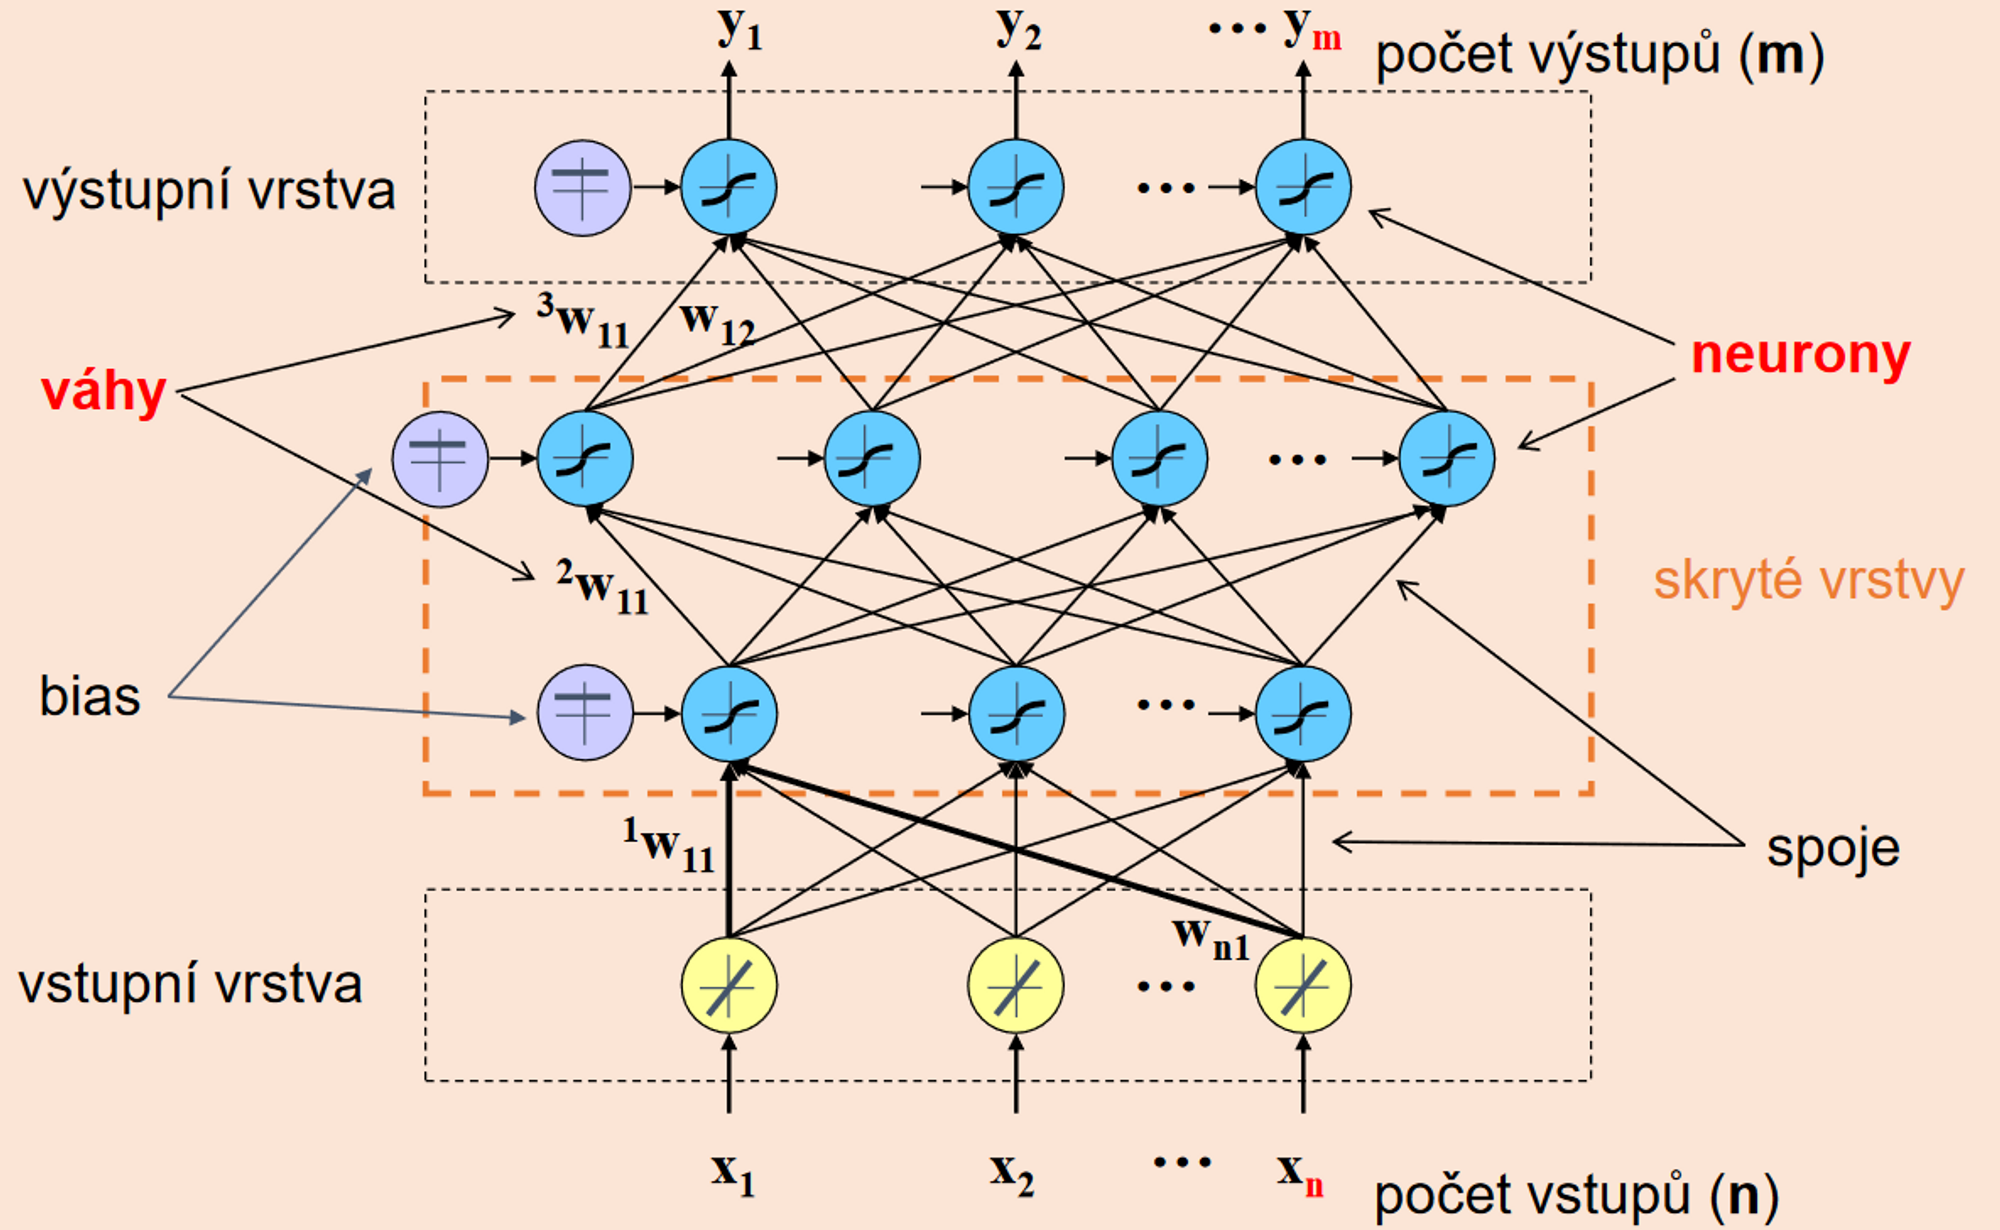
\includegraphics[scale = 0.3]{images/backPropag_topologie.png}
\end{figure}

\subsubsection*{Učení}
učení s učitelem\\
pracuje se s chybou sítě \textit{E}, což je rozdíl mezi skutečnými a požadovanými hodnotami\\
Kroky učení:
\begin{figure}[H]
    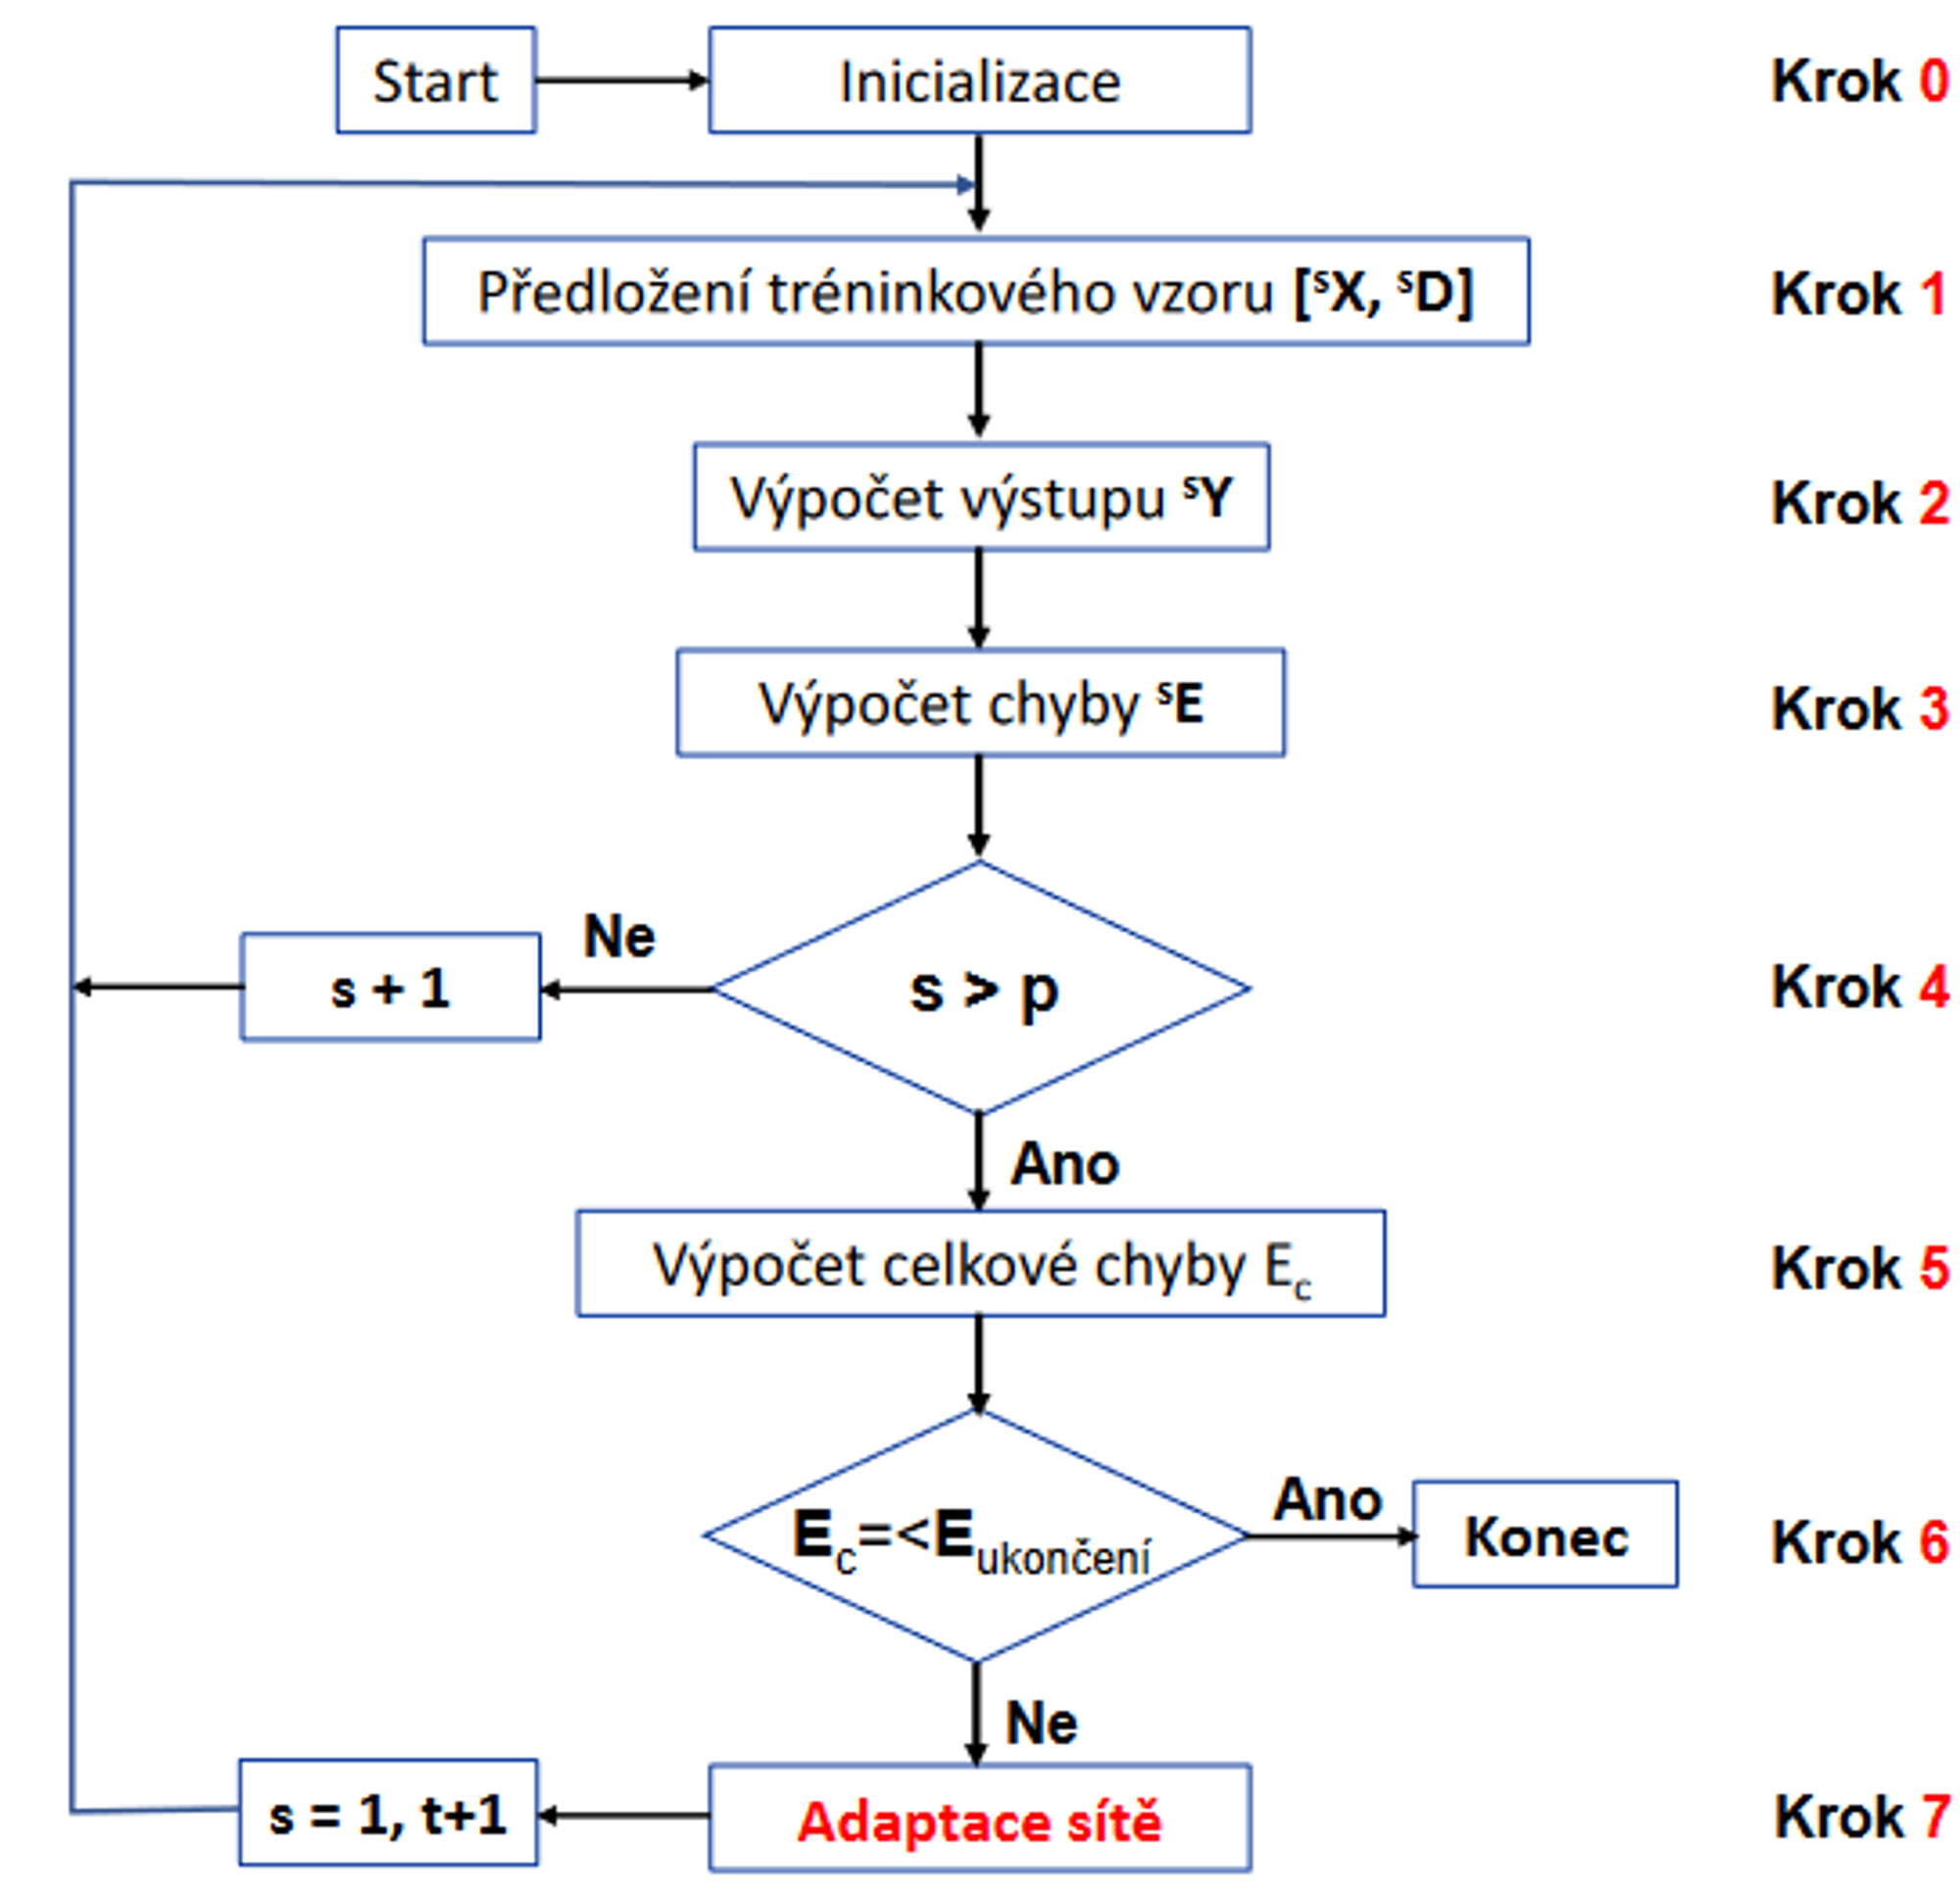
\includegraphics[scale = 0.3]{images/backPropag_uceni.png}
\end{figure}
s \dots počet tréninkových vzorů\\
p \dots celkový počet tréninkových vzorů\\
Akumulované učení - adaptace vah po předložení všech t. vzorů, nezáleží na pořadí vzorů\\
Adaptace po každém tréninkovém vzoru - záleží na pořadí vzorů, zpomaluje konvergenci

\subsection*{Kohonenova samoorganizační mapa}
soutěžní strategie učení\\
nástroj pro identifikaci neznámých vlastností a parametrů skrytých ve vstupních datech(rozmisťování zboží podle toho, jak lidi nakupují)\\
Charakteristika:
\begin{itemize}
    \item neuron - lineární, měření vzdálenosti
    \item topologie - dvouvrstvá s definovaným okolá ve 2.vrstvě
    \item učení - iterační proces, bez učitele
    \item vybavování - jednorázový proces
    \item apliakce - hodně naměřených dat
\end{itemize}
\subsubsection*{Neuron}
ve vstupní vrstvě lineární přenosová funkce\\
ve výstupní není přenosová funkce, zde se provádí výpočet vzdálenosti d
\begin{equation}
    d_j = \sum^n_{i=1} \left(x_i - w_{ij}(t)\right)^2 
\end{equation}
\subsubsection*{Topologie}
Dvouvrstvá síť s úplným propojení neuronů\\
výstupní vrstva je kompetiční\\
\begin{figure}[H]
    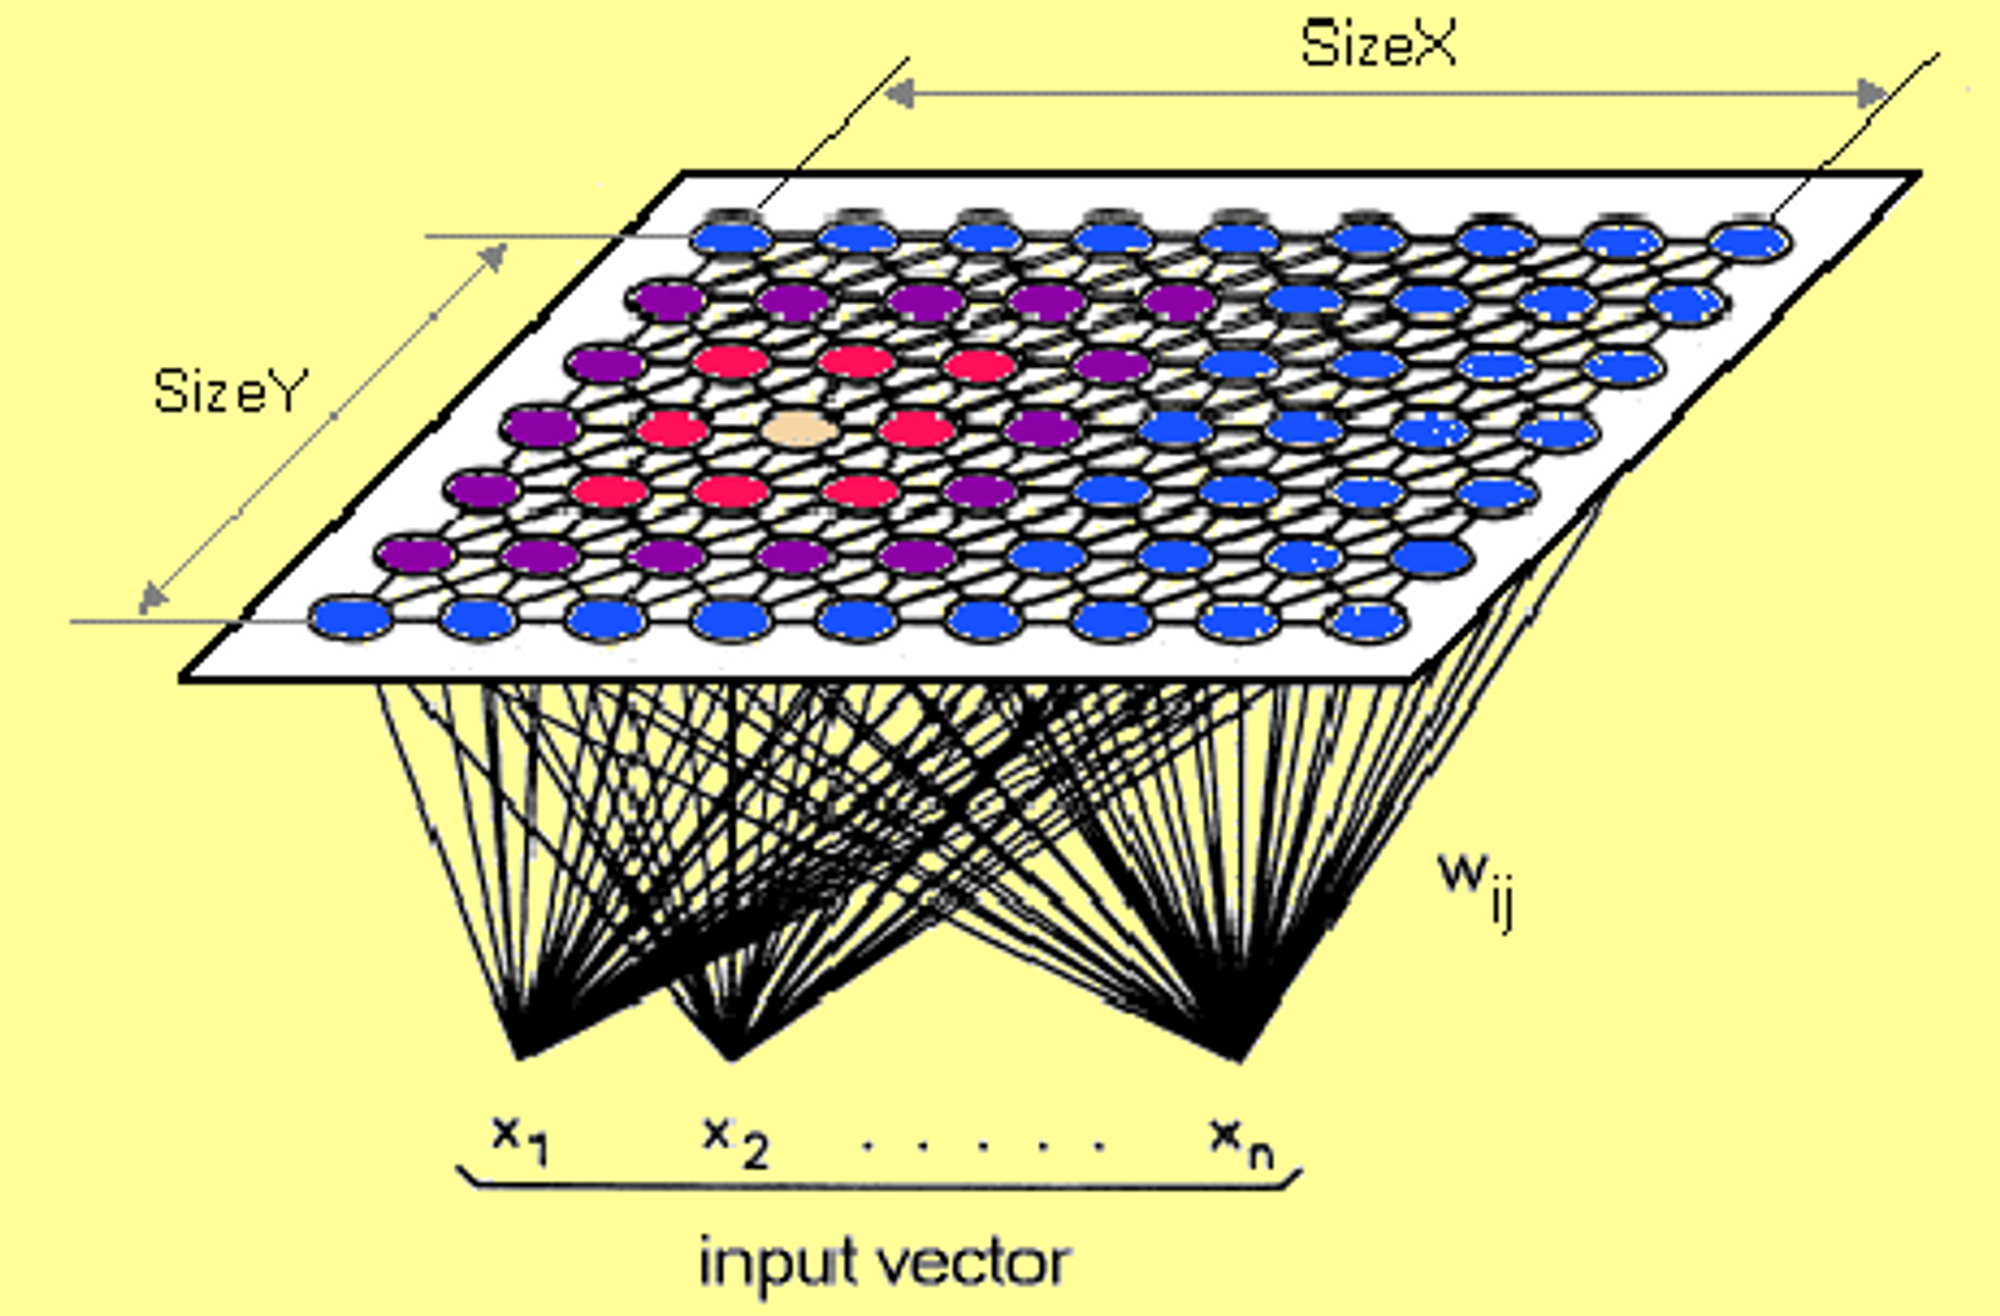
\includegraphics[scale = 0.3]{images/kohonen_topologie.png}
\end{figure}
\newpage
struktura určuje, které neurony spolu sousedí:
\begin{figure}[H]
    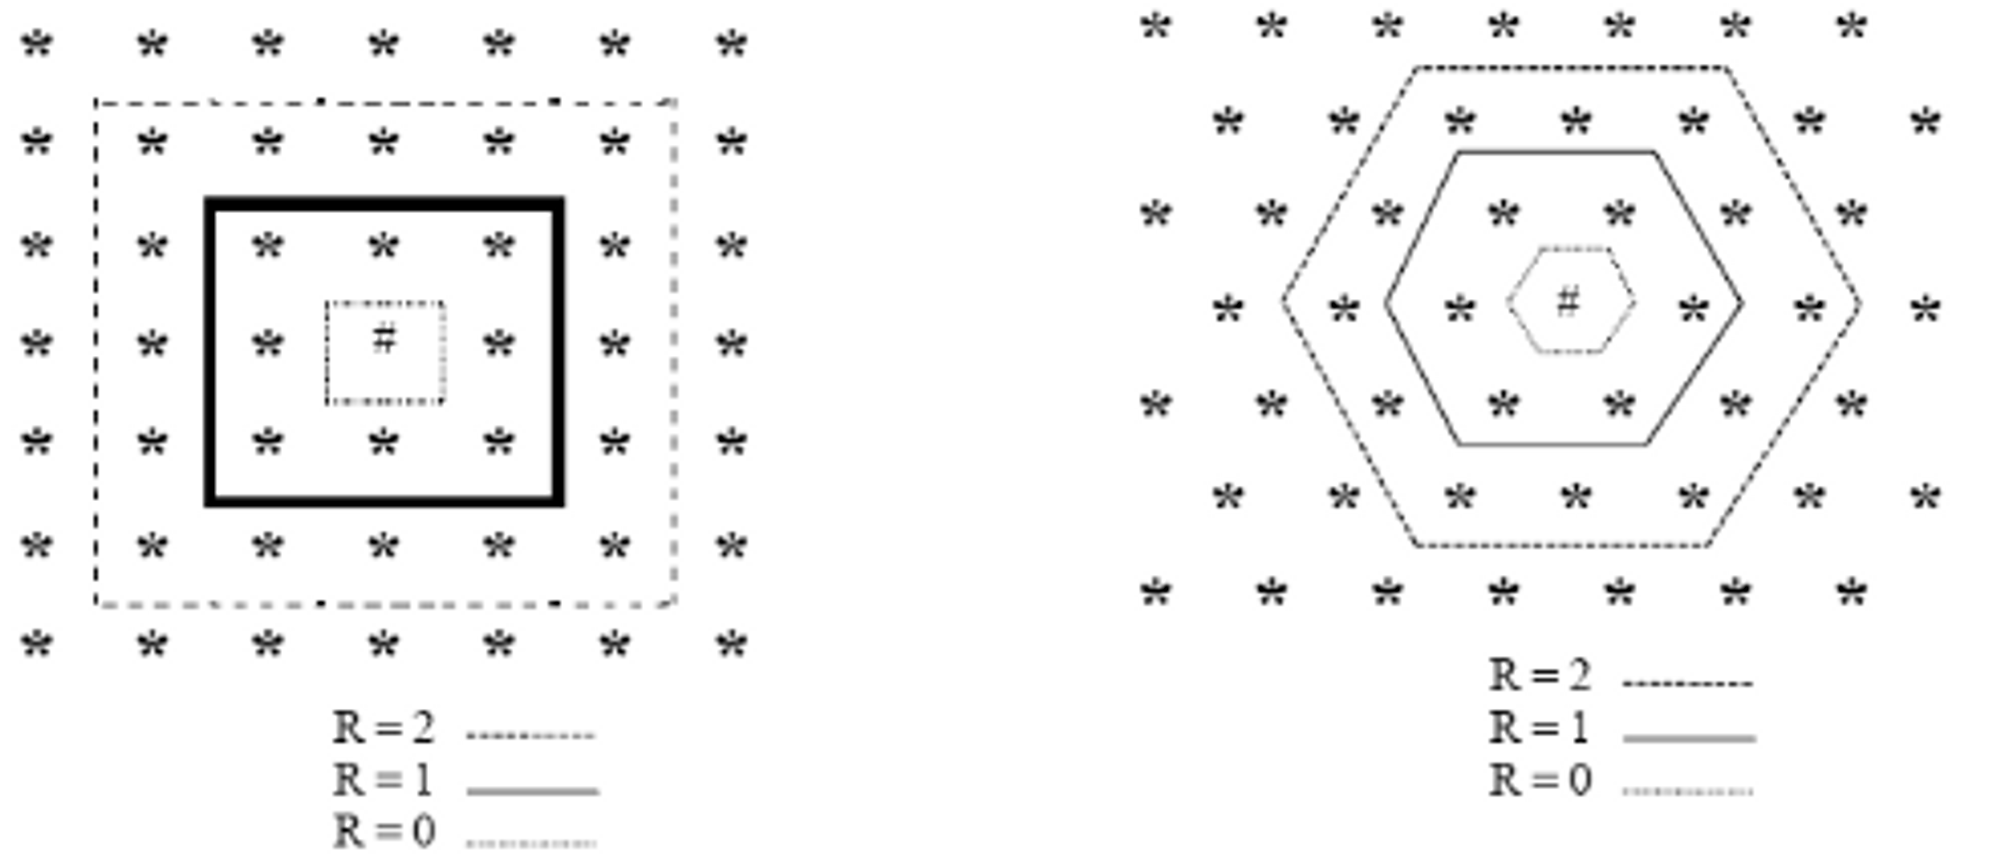
\includegraphics[scale = 0.3]{images/kohonen_struktura.png}
\end{figure}

\subsubsection*{Učení}
Váha úspěšného neuronu je zvýšena, neúspěšných je snížena\\
bez učitele\\
učení probíhá tak, že se umístí neurony kolem jednoho bodu v prostoru(grandmother cell), následně se předloží vstupní data a najde se neuron s nejmenší vzdáleností do tréninkového vzoru, který je vítěz\\
probíhá jednou pro každý tréninkový vzor\\

\subsubsection*{Vybavování}
\begin{enumerate}
    \item předložení vzoru
    \item výpočet vzdáleností
    \item nalezení vítězného neuronu
\end{enumerate}

\subsubsection*{aplikace}
\begin{itemize}
    \item zpracování řeči, obrazu
    \item hledání a detekce osob podle fotografií
    \item přepis ručně psaného textu na tištěný
    \item automatické třídění 
\end{itemize}
\newpage
\subsection*{Konvoluční neuronová síť}
Typické využití u zpracování obrazu\\
Konvoluce je matematický operátor pro spojování dvou funkcí.\\
Má konvoluční jádro, kterým prochází každý prvek obrazu/pole\\
Topologie vícevrstvá neuronová síť\\
Vstupní obraz se musí většinou zkomprimovat pomocí konvoluce a poolingu\\

\begin{figure}[H]
    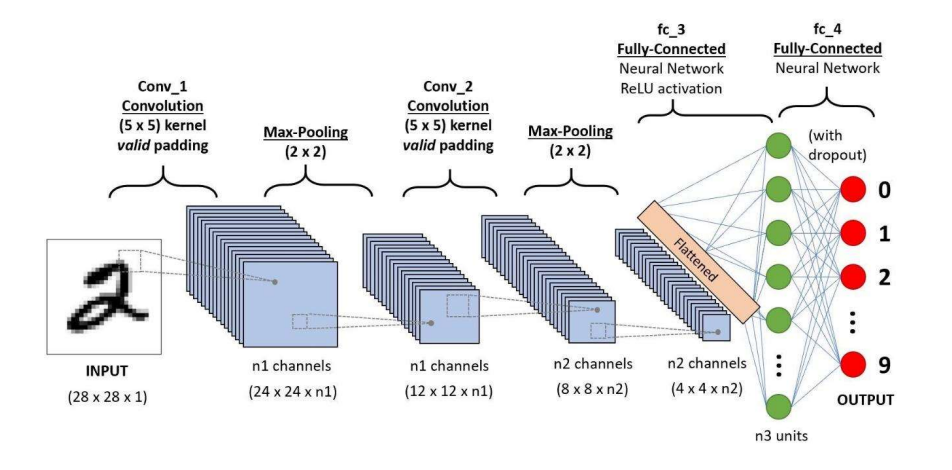
\includegraphics[scale = 1]{images/konvoluce.png}    
\end{figure}